\documentclass[11pt]{article}
\usepackage[utf8]{inputenc}
\usepackage[spanish]{babel}
\usepackage[]{amsthm}
\usepackage{amsmath}
\usepackage[]{amssymb}
\usepackage{graphicx}
\usepackage{wrapfig}
\usepackage[letterpaper, margin=1.5in]{geometry}
\usepackage[hidelinks]{hyperref}
\decimalpoint

\usepackage{pdflscape}

\begin{document}
    \begin{titlepage}
        \begin{center}
            \begin{figure}
                \centering
                
\includegraphics[scale=0.13]{../../img/logo_itesm.png}\\ % Logo de la institución
            \end{figure}
        \vspace{5cm}
        \LARGE{Instituto Tecnológico y de Estudios Superiores de Monterrey}\\
        \fontsize{12}{14}\selectfont
        \vspace{1cm}
        \textbf{Actividad 3.2. Configuración de Firewalls usando Políticas Basadas en Zonas }\\ % Nombre de la tarea
        \vspace{0.7cm}
        \begin{table}[!h]
            \centering
            \begin{tabular}{ ||c|c|| }
                \hline
                Nombre & Matrícula \\
                \hline
                Julio Avelino Amador Fernández & A01276513 \\
                \hline
                Juan Pablo Echeagaray González & A00830646 \\
                \hline
                Verónica Victoria García De la Fuente & A00830383 \\
                \hline
                Erika Martínez Meneses & A01028621 \\
                \hline
                Emily Rebeca Méndez Cruz & A00830768 \\
                \hline
                Ana Paula Ruiz Alvaro & A01367467 \\
                \hline
            \end{tabular}
        \end{table}
        \vspace{0.7cm}
        Análisis de Criptografía y Seguridad\\ % Materia
        \vspace{0.2cm}
        MA2002B.300\\ % Clave de la materia
        \vspace{0.2cm}
        Dr. Alberto Francisco Martínez Herrera \\ % Nombre del profesor
        \vspace{0.7cm}
        5 de junio de 2022\\ % Fecha de entrega
        \end{center}
    \end{titlepage}

    \section{Procedimiento}

        Los ZPF son lo último en la evolución de las tecnologías de firewalls desarrolladas por Cisco. El objetivo de esta actividad es configurar un firewall basado en políticas de zona (ZPF), esto se hace usando la tabla de direccionamiento que se proporcionó, así como el archivo de Packet Tracer diseñado por \emph{Cisco Networking Academy} \cite{security-2018}.

        Para comenzar a realizar el trabajo se descargó el archivo que se encuentra en la plataforma Canvas, en este se dan los datos de pre-configuración de los sistemas en la red, los cuales son los siguientes: 
        
        \begin{itemize}
            \item Contraseña de la consola: \texttt{ciscoconpa55}
            \item Contraseña para lineas vty: \texttt{ciscovtypa55}
            \item Enable password: \texttt{ciscoenpa55}
            \item Nombres de anfitriones y direcciones IP
            \item Nombre de usuario y contraseña local: \texttt{Admin / Adminpa55}
            \item Enrutamiento estático
        \end{itemize}

        \subsection{Verificación de conectividad}

            Antes de implementar el firewall, se verifica el estado de la conexión en la red. Primero se realizó un ping desde la \texttt{PC-A} hacia la \texttt{PC-C} con el IP asociado \texttt{192.168.3.3}. El resultado fue exitoso como se puede ver en la figura \ref{fig:part1-step1}.

            Después se usa Secure Shell para acceder al \texttt{Router 2} desde \texttt{PC-C}. Se conectó a la interfaz \texttt{s0/0/1} con el IP \texttt{10.2.2.2}; cuando se realiza este proceso es necesario proporcionar la contraseña de administrador dada en la documentación de la tarea. La conexión fue exitosa como se puede ver en la figura \ref{fig:part1-step2}.

            Finalmente, se prueba la conexión entre la \texttt{PC-C} y el servidor \texttt{PC-A} por medio del buscador de la computadora. Dentro del navegador se captura el IP asociado al servidor \texttt{192.168.1.3}, se espera que se despliegue una imagen como la que presentamos en la figura \ref{fig:part1-step3}.

        \subsection{Creación de las zonas del Firewall}

            Se inicia el proceso de creación del firewall verificando que el paquete \texttt{Security Technology} esté habilitado. Usando el comando \texttt{show version} dentro del \texttt{Router 3} en su modo de configuración se despliega un resumen del estado del router; al final se presenta un tabulado como en la figura \ref{fig:part2-step1}, nótese que en la fila con la celda \texttt{security} no hay ningún paquete habilitado.

            Para habilitarlo se debe de correr el comando \texttt{license boot module c1900 technology-package securityk9} dentro del mismo router en su modo de configuración. Se acepta el acuerdo de usuario, se guardan las modificaciones y se reinicia el router. Para verificar que los cambios realizados han tomado efecto, se usa de nuevo el comando \texttt{show version}, ahora este producirá un resultado como el presentado en la figura \ref{fig:part2-step1b}.

            Ahora que se tiene habilitado el paquete de seguridad, se crean las zonas \texttt{IN-ZONE} y \texttt{OUT-ZONE}. Esto se realiza con el comando \texttt{zone security ZONE-NAME} en el router en su modo de configuración, al usuario se le pedirán las credenciales pertinentes. Al finalizar este proceso la consola produce un resultado como el de la figura \ref{fig:part2-step23}.

        \subsection{Identificación de tráfico usando Class-Maps}

            Se comienza el proceso de identificado de tráfico con la creación de un \texttt{access list} extendido. Desde el router 3 (en modo configuración) diseñamos un permiso para que cualquier IP proveniente de \texttt{192.168.3.0} pueda pasar a cualquier destino por medio del comando \texttt{access-list 101 permit ip 192.168.3.0 0.0.0.255 any}.

            Después se crea un \texttt{class map} que haga referencia a todo el tráfico interno del \texttt{access list} creado anteriormente, a este mapa se le da el nombre \texttt{IN-NET-CLASS-MAP}, esto se logra con la secuencia de comandos \texttt{class-map type inspect match-all IN-NET-CLASS-MAP}, \texttt{match access-group 101}, \texttt{exit}.

            Los comandos que se corren en esta sección no producen una salida en la consola a menos que haya ocurrido un error, para nuestro caso esto no ha sucedido como se puede ver en la figura \ref{fig:part3}.

        \subsection{Especificación de políticas del Firewall}

            Ya que se tienen el mapa de clases se crea un mapa de políticas para determinar qué sucede con el tráfico que fluye dentro de la red. Dentro del \texttt{Router 3} en su modo de configuración se corre el comando \texttt{policy-map type inspect IN-2-OUT-PMAP}, a esta política después le decimos que tipo de tráfico investigar, le daremos el que se definió en la sección anterior con el comando \texttt{class type inspect IN-NET-CLASS-MAP}. Finalizamos por decirle que queremos que investigue este tráfico con el comando \texttt{inspect}; se guardan estos cambios al correr 2 veces la ejecutiva \texttt{exit}.

            Estos comandos producirán una salida similar a la de la figura \ref{fig:part4}.

        \subsection{Aplicación de políticas del Firewall}

            Una vez que se han especificado las políticas del firewall, debemos de configurar su aplicación. Esto comienza al crear un par de zonas que llamaremos \texttt{IN-2-OUT-ZPAIR}, se configura con el comando \texttt{zone-pair security IN-2-OUT-ZPAIR source IN-ZONE destination OUT-ZONE}.

            Le especificamos que use la política definida en el paso anterior con el comando \texttt{service-policy type inspect IN-2-OUT-PMAP} y se guarda este proceso con el comando \texttt{exit}. Los comandos resultarán en una salida como la presentada en la figura \ref{fig:part5}.

        \subsection{Prueba del funcionamiento del Firewall}

            Para esta etapa el firewall ya ha sido configurado, lo único que resta es comprobar su buen funcionamiento. Verificaremos qué resulta de intentar conectarse del interior del firewall al exterior, y después verificaremos que el tráfico del exterior al interior del firewall es bloqueado.

            \subsubsection{IN-ZONE a OUT-ZONE}

                Hacemos una prueba de conexión entre el equipo \texttt{PC-C} hacia el servidor externo \texttt{PC-A} que tiene el IP asociado \texttt{192.168.1.3}. El resultado del \texttt{ping} se presenta en la imagen \ref{fig:part6-step1}.

                Después desde \texttt{PC-C} se utiliza Secure Shell para conectarse al \texttt{Router 2}; mientras que la conexión esté activa se checa el tráfico que viaja por el \texttt{Router 3} con el comando \texttt{show policy-map type inspect zone-pair}, producirá el resultado que se ve en la figura \ref{fig:part6-step2}.

                Vemos que el IP fuente de la sesión es \texttt{192.168.3.3} y que el de destino es \texttt{10.2.2.2}. Después terminamos la sesión SSH.

                Ahora se realiza la misma prueba del navegador hecha con anterioridad, desde \texttt{PC-C} creamos una conexión desde el navegador hacia \texttt{PC-A}. Se repite el mismo proceso del paso anterior para identificar el tráfico. Como se puede ver en la figura \ref{fig:part6-step4}.

                En este caso vemos que el IP fuente es \texttt{192.168.3.3} y el de destino es \texttt{192.168.1.3}.

            \subsubsection{OUT-ZONE a IN-ZONE}

                Se realiza una prueba de conexión desde \texttt{PC-A} hacia \texttt{PC-C}, esta prueba fallará como se demuestra en la figura \ref{fig:part7-step1}.

                Ahora se prueba la conexión desde el \texttt{Router 2} hacia \texttt{PC-C}, esta prueba también regresará una evidencia de conexión fallida como en la figura \ref{fig:part7-step2}.

        Una vez que se ha realizado todo este proceso y se checan los resultados, el programa arrojará una imagen similar a la de la figura \ref{fig:part7-step3}.

    \section{Conclusiones}  
        Esta actividad fue de bastante utilidad para poder entender mejor el funcionamiento de un firewall ZBP. Con la ayuda del software Packet Tracer, pudimos ver la simulación y el funcionamiento en el mismo y conforme se iba siguiendo el tutorial se fue entendiendo cada comando usado.
    
    \clearpage
    \bibliographystyle{apalike}
    \bibliography{references.bib}

    \appendix
    \section{Capturas de pantalla}

        \begin{figure}[!h]
            \centering
            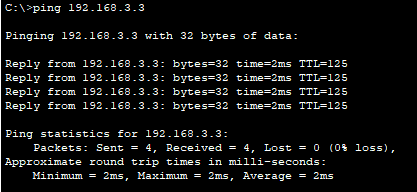
\includegraphics[scale=0.9]{img/part1-step1.png}
            \caption{Prueba de conectividad entre PC-A y PC-C}
            \label{fig:part1-step1}
        \end{figure}

        \begin{figure}[!h]
            \centering
            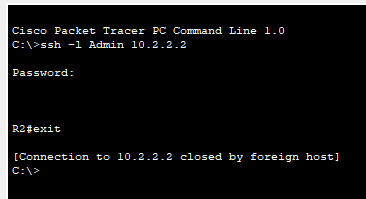
\includegraphics[scale=0.9]{img/part1-step2.png}
            \caption{Prueba de SSH en router 2 desde PC-C}
            \label{fig:part1-step2}
        \end{figure}

        \clearpage
        \begin{figure}[!h]
            \centering
            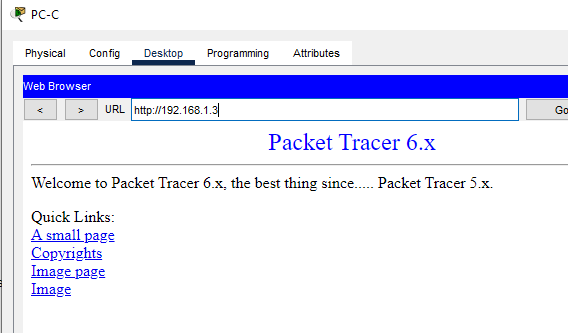
\includegraphics[scale=0.7]{img/part1-step3.png}
            \caption{Prueba del navegador entre PC-C y PC-A}
            \label{fig:part1-step3}
        \end{figure}
        
        \begin{figure}[!h]
            \centering
            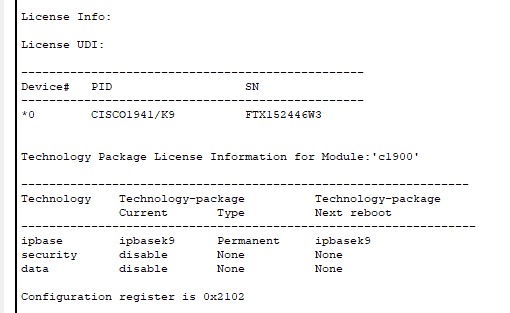
\includegraphics[scale=0.7]{img/part2-step1.png}
            \caption{Verificación de activación de paquete de seguridad en R3}
            \label{fig:part2-step1}
        \end{figure}

        \clearpage
        \begin{figure}[!h]
            \centering
            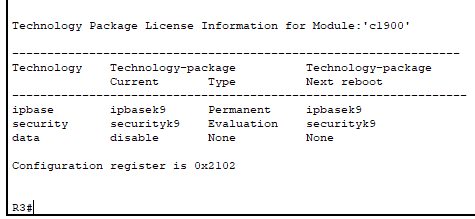
\includegraphics[scale=0.8]{img/part2-step1b.png}
            \caption{Paquete de seguridad habilitado en R3}
            \label{fig:part2-step1b}
        \end{figure}

        \begin{figure}[!h]
            \centering
            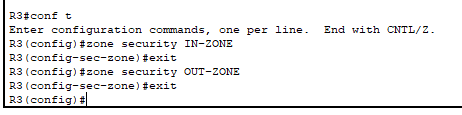
\includegraphics[scale=0.9]{img/part2-step-23.png}
            \caption{Creación de zona interna y externa}
            \label{fig:part2-step23}
        \end{figure}
        
        \begin{figure}[!h]
            \centering
            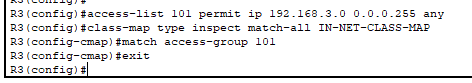
\includegraphics[scale=0.9]{img/part3.png}
            \caption{Creación del class-map para el firewall}
            \label{fig:part3}
        \end{figure}
        
        \clearpage
        \begin{figure}[!h]
            \centering
            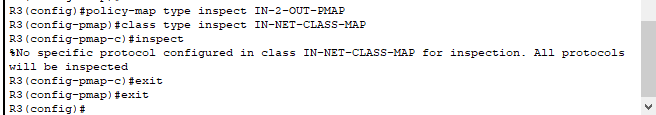
\includegraphics[scale=0.85]{img/part4.png}
            \caption{Especificación de las políticas del firewall}
            \label{fig:part4}
        \end{figure}

        \begin{figure}[!h]
            \centering
            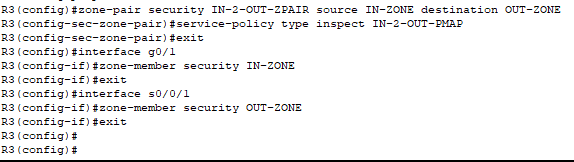
\includegraphics[scale=0.85]{img/part5.png}
            \caption{Aplicación de las políticas del firewall}
            \label{fig:part5}
        \end{figure}
        
        \clearpage
        \begin{figure}[!h]
            \centering
            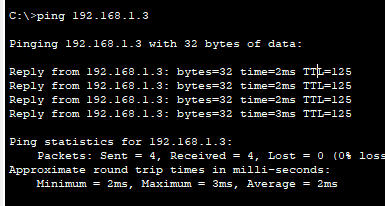
\includegraphics[scale=0.9]{img/part6-step1.png}
            \caption{Prueba de conexión entre PC-C y PC-A}
            \label{fig:part6-step1}
        \end{figure}

        \begin{figure}[!h]
            \centering
            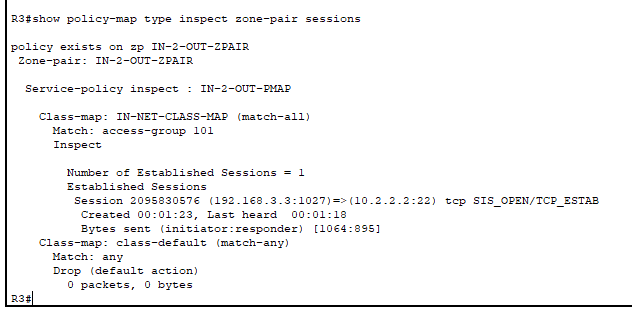
\includegraphics[scale=0.8]{img/part6-step2.png}
            \caption{Chequeo 1 de sesiones activas a través de R3}
            \label{fig:part6-step2}
        \end{figure}

        \clearpage
        \begin{figure}[!h]
            \centering
            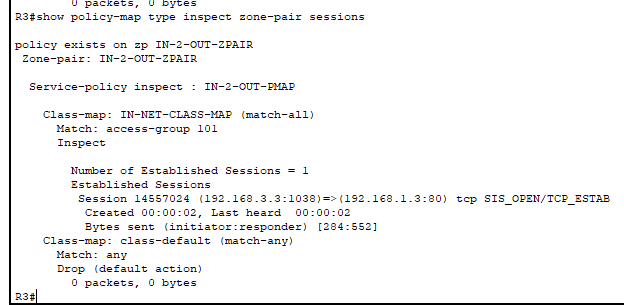
\includegraphics[scale=0.8]{img/part6-step4.png}
            \caption{Chequeo 2 de sesiones activas a través de R3}
            \label{fig:part6-step4}
        \end{figure}

        \begin{figure}[!h]
            \centering
            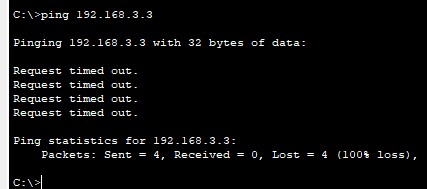
\includegraphics[scale=0.8]{img/part7-step1.png}
            \caption{Prueba de conexión desde PC-A hacia PC-C}
            \label{fig:part7-step1}
        \end{figure}

        \begin{figure}[!h]
            \centering
            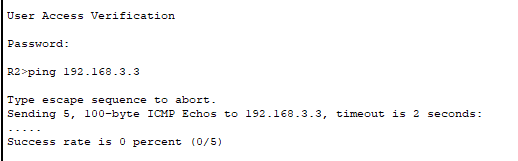
\includegraphics[scale=0.8]{img/part7-step2.png}
            \caption{Prueba de conexión desde R2 hacia PC-C}
            \label{fig:part7-step2}
        \end{figure}
        
        \begin{landscape}
            \begin{figure}[!h]
                \centering
                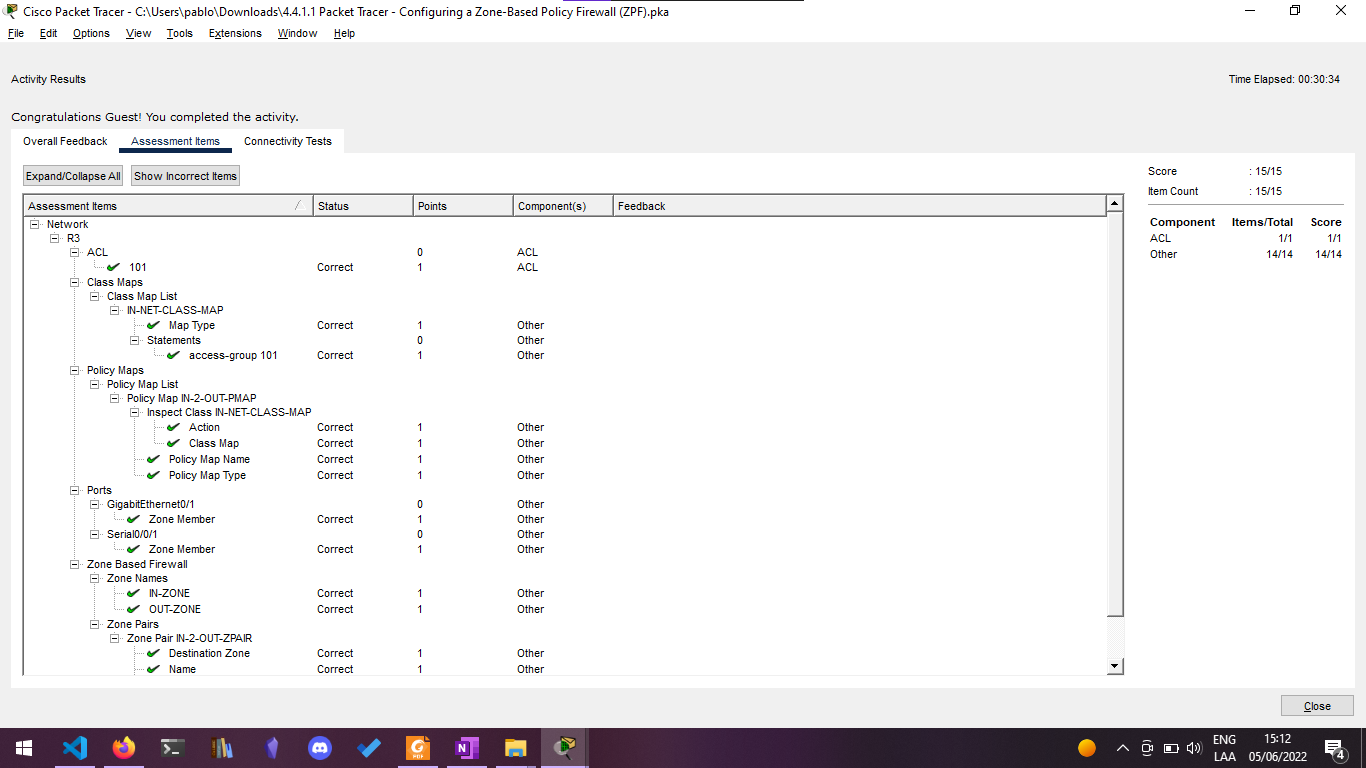
\includegraphics[scale=0.5]{img/part7-step3.png}
                \caption{Evidencia de finalización de actividad}
                \label{fig:part7-step3}
            \end{figure}
        \end{landscape}

\end{document}